\documentclass{standalone}

\usepackage{tikz}
    \usetikzlibrary{arrows.meta}
    \usetikzlibrary{calc}

% \pagecolor{black}
\color{white}

\tikzset{
    pics/box frame/.style args={(#1+#2)x#3}{
        code={
            \draw rectangle (#3,#1);
            \draw rectangle (#3,-#2);
        }},
}



\begin{document}
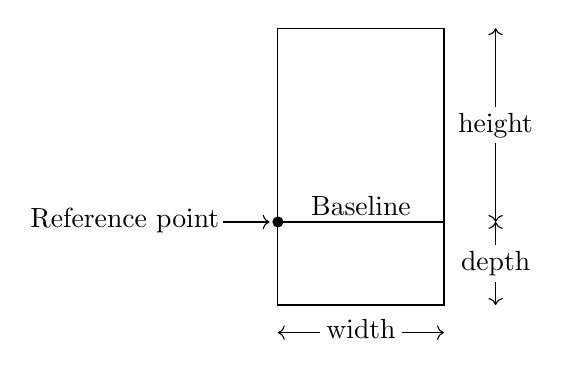
\begin{tikzpicture}[x=1pt, y=1pt]

    \def\boxh{70}
    \def\boxd{30}
    \def\boxw{60}

    \pic {box frame=(\boxh+\boxd)x\boxw};
    \fill circle [radius=2pt];

    \begin{scope}[inner sep=2pt]
        \node[below=3pt] (W) at (\boxw/2, -\boxd)  {width} ;
        \node[right=3pt] (H) at (\boxw, \boxh/2) {height};
        \node (D) at (0,-\boxd/2 -| H) {depth} ;
        \node[above] (B) at (\boxw/2,0) {Baseline};
        \node[anchor=base east, yshift=-0.5ex, xshift=-20pt, inner sep=1pt] (R) at (0,0) {Reference point};
    \end{scope} 

    \draw[<-] (0,0.5ex) +(0,0 |- W.base west) -- +(W.base west);
    \draw[->] (0,0.5ex) +(W.base east) -- +(\boxw,0 |- W.base east);
    \draw[<-] (0,0 -| H.south) -- (H.south);
    \draw[->] (H.north) -- (0,\boxh -| H.south);
    \draw[<-] (0,-\boxd -| D.south) -- (D.south);
    \draw[->] (D.north) -- (0,0 -| D.south);
    \draw[->] (0,0.5ex) +(R.base east) -- +(R.base east -| -3pt,0);
    
\end{tikzpicture}
\end{document}